\chapter{Opis opšte AST apstrakcije za imperativne jezike}
\label{chp:MyAST}

Broj različitih stilova programiranja je veliki i moderni programski jezici se često ne pripadaju striktno jednom stilu. Zbog ove raznovrsnosti, apstrahovati svaki programski jezik je težak podvig, ako je uopšte i moguće dovesti fundamentalno različite koncepte na isti nivo apstrakcije. Stoga će u ovom radu biti apstrahovan samo imperativni stil programiranja, međutim zbog načina na koji je imperativno programiranje evoluiralo, moderni imperativni programski jezici često pružaju i proceduralne ali i funkcionalne koncepte. Stoga će u odeljku \ref{sec:Paradigms} biti više reči o popularnim stilovima programiranja, dok će u odeljku \ref{sec:MyAST} biti više reči o apstrakciji imperativnog stila programiranja ali i njegovih derivata: strukturnog, proceduralnog i OO stila.

\section{Programske paradigme}
\label{sec:Paradigms}

Iako se u suštini svode na mašinski jezik ili asembler, viši programski jezici mogu imati velike razlike međusobno --- kako u načinu pisanja koda, tako i u efikasnosti izvršavanja. Način, ili stil programiranja se naziva \emph{programska paradigma} \cite{ProgrammingParadigms}. Može se pokazati da sve što je rešivo putem jedne, može da se reši i putem ostalih; međutim neki problemi se prirodnije rešavaju koristeći specifične paradigme. Neke poznatije programske paradigme su navedene u nastavku zajedno sa njihovim odlikama i primerima upotrebe.


\subsection{Imperativna paradigma}
\label{subsec:ParadigmImperative}

\emph{Imperativna paradigma} pretpostavlja da se promene u trenutnom stanju izvršavanja mogu sačuvati kroz promenljive. Izračunavanja se vrše putem niza koraka, u svakom koraku se te promenljive referišu ili se menjaju njihove trenutne vrednosti. Raspored koraka je bitan, jer svaki korak može imati različite posledice s obzirom na trenutne vrednosti promenljivih na početku tog koraka. Primer koda pisanog u imperativnoj paradigmi se može videti na slici \ref{fig:ParadigmImperative}.

\begin{figure}[h!]
\begin{lstlisting}
    result = []
    i = 0
start:
    numPeople = length(people)
    if i >= numPeople goto finished
    p = people[i]
    nameLength = length(p.name)
    if nameLength <= 5 goto nextOne
    upperName = toUpper(p.name)
    addToList(result, upperName)
nextOne:
    i = i + 1
    goto start
finished:
    return sort(result)
\end{lstlisting}
\caption{Primer koda pisanog u imperativnoj paradigmi.}
\label{fig:ParadigmImperative}
\end{figure}

Stariji programski jezici najčešće prate ovu paradigmu iz nekoliko razloga. Prvi je taj što imperativna paradigma najbliže oslikava samu mašinu na kojoj se program izvršava, pa je programer mnogo bliži mašini. Ova paradigma je bila veoma popularna zbog ranih ograničenja u hardveru i potrebe za efikasnim programima. Danas, zbog mnogo bržeg razvoja i mnogo jačih računara, efikasnost dobijena pisanjem koda u jezicima veoma bliskim mašini se sve manje uzima u obzir.

Imperativna paradigma svoje nedostatke. Naime, najveći problem je razumevanje i verifikovanje ispravnosti programa zbog postojanja propratnih efekata\footnote{Propratni efekti (promena stanja mašine) ne poštuju \emph{referencijalnu transparentnost} koja se definiše na sledeći način: \emph{Ako važi $P(x)$ i $x = y$ u nekom trenutku, onda $P(x) = P(y)$ važi tokom čitavog vremena izvršavanja programa}.}. Stoga je zahtevno i pronalaženje grešaka u programima pisanim u imperativnoj paradigmi. Pošto je k\^od veoma niskog nivoa, obično je dozvoljen i direktan pristup memorijskim adresama putem \emph{pokazivača}, što takođe otežava verifikaciju koda.


\subsection{Strukturna paradigma}
\label{subsec:ParadigmImperativeStructural}

\emph{Strukturna paradigma} je vrsta imperativne paradigme gde se kontrola toka vrši putem niza naredbi, uslovnih grananja i petlji. Promenljive su obično lokalne za blok u kome su definisane, što određuje i njihov životni vek i vidljivost. Primer koda pisanog u strukturnoj paradigmi se može videti na slici \ref{fig:ParadigmStructural}. Danas je najpopularnija kombinacija strukturne paradigme sa \emph{proceduralnom paradigmom}, baziranom na konceptu poziva \emph{procedure} --- podrutine ili funkcije koja sadrži seriju koraka koje je potrebno izvršiti redom.

\begin{figure}[h!]
\begin{lstlisting}
result = [];
for (i = 0; i < length(people); i++) {
    p = people[i];
    if (length(p.name)) > 5 {
        addToList(result, toUpper(p.name));
    }
}
return sort(result);
\end{lstlisting}
\caption{Primer koda pisanog u strukturnoj paradigmi.}
\label{fig:ParadigmStructural}
\end{figure}


\subsection{Skript paradigma i njen odnos sa proceduralnom paradigmom}
\label{subsec:Languages}

Čak i unutar jedne paradigme kao što je proceduralna, mogu se naći veoma velike varijacije u izgledu koda pisanog u različitim programskim jezicima. Kako hardver postaje moćniji, više se ceni vreme koje programer provede u procesu pisanja koda nego koliko je taj k\^od efikasan. Štaviše, u nekim slučajevima je dobitak u efikasnosti veoma mali u poređenju sa vremenom koje je potrebno utrošiti da bi se ta efikasnost postigla. Ukoliko se program pokreće veoma retko, možda nije ni bitno da li se on izvršava sekundu sporije od efikasnog programa, ako je za njegovo pisanje utrošeno znatno manje vremena. Ovo je pristup koji prate \emph{skript} jezici kao što su \texttt{Python, Lua, Perl, bash} itd. Iako proceduralni, oni se razlikuju od klasičnih predstavnika proceduralne paradigme i njihove razlike su vremenom postale tolike da se skript jezici obično svrstavaju u zasebnu, \emph{skript paradigmu}. Stoga će se u nastavku pod terminom \emph{proceduralni jezik} smatrati tradicionalni proceduralni jezik, ukoliko nije naznačeno drugačije. Na slici \ref{fig:LanguagesDiff} se mogu uočiti navedene razlike.

\begin{figure}[h!]
\begin{lstlisting}
int main() {
    int k = 0;
    for (int i = 0; i < 1000000; i++)
        k++;
    return 0;
}
\end{lstlisting}
\begin{lstlisting}[language={}]
$ time: 0.03s user 0.00s system 70% cpu 0.044 total
\end{lstlisting}
\begin{lstlisting}
k = 0
for i = 0, 1000000 do 
    k = k + 1 
end
\end{lstlisting}
\begin{lstlisting}[language={}]
$ time: 0.17s user 0.03s system 92% cpu 0.203 total
\end{lstlisting}
\caption{Primer koda pisanog u tradicionalnoj proceduralnoj paradigmi (gore, \texttt{C}) i u modernoj skript paradigmi (dole, \texttt{Lua}) kao i odgovarajuća vremena izvršavanja dobijena komandom \texttt{time}.}
\label{fig:LanguagesDiff}
\end{figure}

Promenljive predstavljaju jedan od osnovnih koncepata na kojem se zasnivaju i proceduralni i skript jezici. Promenljivu odlikuje, između ostalog, i njen \emph{tip} koji određuje količinu memorije potrebnu za njeno skladištenje. Proceduralni programski jezici najčešće zahtevaju eksplicitno definisanje tipa promenljive u kodu jer su većinom \emph{statički tipizirani}, što znači da se tipovi promenljivih određuju u fazi prevođenja --- posledica toga je da promenljive ne mogu menjati svoj tip tokom izvršavanja programa. Proces uvođenja imena za memorijsku lokaciju koja predstavlja mesto skladištenja vrednosti promenljive određenog tipa se naziva \emph{deklaracija promenljive}. Slično kao i za promenljive, potrebno je deklarisati i funkcije pre trenutka njihovog korišćenja kako bi prevodilac znao broj i tipove parametara funkcije kao i njihove povratne vrednosti. Skript jezici su, za razliku od proceduralnih, najčešće \emph{dinamički tipizirani}, što znači da tipovi promenljivih zavise od trenutnih vrednosti promenljviih u fazi izvršavanja. Stoga je proces pisanja koda u dinamički tipiziranim jezicima brži jer se ne moraju navesti tipovi promenljivih\footnote{U nekim programskim jezicima koji su statički tipizirani (npr.~Haskell) prevodilac može da zaključi tip na osnovu konteksta u kom se promenljiva koristi, stoga programer ne mora da eksplicitno navede tipove funkcija. Takođe, većina skript jezika dozvoljava eksplicitno definisanje tipa, ali to nije neophodno da bi se k\^od preveo.}. Slično, parametri i povratne vrednosti funkcija takođe ne moraju biti fiksnog tipa.

Kod statički tipiziranih proceduralnih jezika, mogu se koristiti strukture podataka koje omogućavaju brz pristup svojim elementima. To su na primer nizovi koji predstavljaju kontinualni blok memorije u kom su elementi niza smešteni jedan do drugog. Pristup se vrši na osnovu indeksa i, pošto su svi elementi istog tipa (zauzimaju jednaku količinu memorije), može se u konstantnom vremenu izračunati memorijska lokacija na kojoj se nalazi element niza sa datim indeksom. Kompleksnije strukture podataka obično nisu podržane u samom jeziku. Neki proceduralni jezici dozvoljavaju veoma niski pristup kroz \emph{pokazivače} ili \emph{reference} na memorijske adrese (npr. \texttt{C}, \texttt{C++}, \texttt{Go}, \texttt{Rust}). Većina modernih proceduralnih jezika (npr. \texttt{Java}, \texttt{JavaScript}. \texttt{Python}, \texttt{Lua}) ne dozvoljava korišćenje pokazivača, dok neki to dozvoljavaju ali sa eksplicitnom naznakom (\texttt{C\#}).

Pored dinamičnosti kad je u pitanju tip promenljivih, skript jezici često imaju neke specifične strukture podataka ugrađene u sam jezik kao olakšice prilikom programiranja. Za razliku od proceduralnih jezika gde su osnovne strukture podataka često kontinualni blokovi memorije sa proizvoljnim pristupom po indeksu, primarna struktura podataka kod skript jezika je najčešće \emph{jednostruko ulančana lista}\footnote{Lista je rekurzivna kolekcija podataka koja se sastoji od glave koja sadrži vrednost određenog tipa, i pokazivača na rep --- drugu listu. Specijalno, praznim pokazivačima se označava kraj liste (prazna lista).}. Razlog zašto se koriste liste je delimično zbog toga što, kao i ostale promenljive, liste ne moraju da budu statički tipizirane. Moguće je u listu ubacivati elemente različitih tipova --- što onemogućava skladištenje u kontinualnom bloku memorije (osim ukoliko je lista nepromenljiva, što obično nije slučaj). Skript jezici uglavnom omogućavaju indeksni pristup elementima liste, pa programeru izgleda kao da radi nad običnim nizom. Neki skript jezici omogućavaju kreiranje \emph{asocijativnih nizova}, gde indeks niza ne mora biti ceo broj već može uzimati vrednost iz domena bilo kog tipa. Osim listi, obično su podržane i \texttt{torke}\footnote{Torka (engl. \emph{tuple}) je nepromenljiva, uređena struktura podataka koja predstavlja sekvencu elemenata.}, i za njih važe iste slobode kao i za liste. Kompleksnije strukture podataka uključuju skupove i rečnike ili \emph{mape} (engl. \emph{dictionaries, maps}) koji predstavljau kolekciju ključ-vrednost parova gde je dozvoljen indeksni pristup vrednosti para koristeći ključ. Razne implementacije mapa postoje i u proceduralnim jezicima, ali ključna razlika je ta što tipovi u skript jezicima nisu striktni --- ključevi međusobno, ali i vrednosti mogu biti različitog tipa. Vredi naglasiti da se mape mogu porediti sa objektima određenih klasa --- svaki objekat se može serijalizovati u mapu gde su ključevi imena javnih atributa klase a vrednosti su vrednosti javnih atributa objekta koji se serijalizuje. Neki jezici (kao što je Python), imaju funkcije koje od objekta vraćaju baš ovakvu mapu. U programskom jeziku Lua, asocijativni nizovi (tzv. \emph{tabele}) implementiraju sve ostale strukture podatake, pa i klase, što direktno odgovara ideji poređenja objekata sa rečnicima odnosno asocijativnim nizovima.

Skript programski jezici su skoro uvek interpretirani, iako se neki jezici mogu kompilirati po potrebi za efikasnije ponovno izvršavanje. S obzirom da efikasnost nije u glavnom planu, u skript jezicima nije dozvoljen direktan pristup memoriji putem pokazivača ili referenci. 


\subsection{OO paradigma i njen odnos sa proceduralnom paradigmom}
\label{subsec:ParadigmOOP}

\emph{Objektno-orijentisana paradigma} (kraće \emph{OOP} ili \emph{OO paradigma}) je paradigma u kojoj se objekti stvarnog sveta posmatraju kao zasebni entiteti koji imaju sopstveno stanje koje se modifikuje samo pomoću procedura ugrađenih u same objekte --- tzv. \emph{metode}. Pošto objekti operišu nezavisno jedni od drugih, moguće je enkapsulirati ih u module koji sadrže lokalnu sredinu i metode dok se komunikacija sa objektom vrši prosleđivanjem poruka. Objekti su organizovani u klase, od kojih nasleđuju atribute i metode. OO paradigma omogućava ponovno korišćenje i jednostavnu proširivost koda. Primer koda pisanog u OO paradigmi se može videti na slici \ref{fig:ParadigmOO}.

\begin{figure}[h!]
\begin{lstlisting}
class Person
{
    private string name;
    private int wage;
    private int income = 0;

    Person(string name, int wage) {
        this.name = name;
        this.wage = wage;
    }

    public void Work(int hours) {
        this.income += hours * this.wage;
    }
}

Person p1 = new Person("John Doe", 30);
Person p2 = new Person("Dave Doe", 35);
p1.Work(7);
p2.Work(8);
\end{lstlisting}
\caption{Primer koda pisanog u OO paradigmi.}
\label{fig:ParadigmOO}
\end{figure}

Iako se OOP posmatra kao zasebna paradigma, moderni programski jezici često koriste OO koncepte iako nisu nužno predstavnici OO paradigme. Jedan od primera je i programski jezik \texttt{Python} koji, iako svrstan u skript paradigmu, pruža i OO koncepte kao što su klase, metode i nasleđivanje. Razlog za ovo je najviše prednost koje OO paradigma pruža ukoliko se radi na velikim programima, ali i taj što implementacija metoda OO klasa podseća na proceduralni k\^od. Neki programski jezici kao što je \texttt{Lua} nemaju koncept klase, ali imaju koncept nasleđivanja. U ovom radu neće biti implementirane apstrakcije OO koncepata kao što su klase ili interfejsi.

\subsection{Ostale popularne programske paradigme}
\label{subsec:ParadigmsOther}

\emph{Logička paradigma} koristi deklarativni pristup rešavanju problema i po tome se razlikuje od ostalih paradigmi opisanih u ovom odeljku. Umesto zadavanja instrukcija koje treba da dovedu do rezultata, opisuje se sam rezultat kroz činjenice --- skup logičkih pretpostavki koji se zatim prevodi u upit koji se dalje koristi. Uloga računara je održavanje skupa poznatih činjenica i logička dedukcija korišćenjem skupa poznatih činjenica iz koje proizilaze nove činjenice koje su od značaja za rešavanje problema. 

\emph{Funkcionalna paradigma} posmatra sve potprograme kao funkcije u matematičkom smislu --- uzimaju argumente i vraćaju jedinstven rezultat. Povratna vrednost zavisi isključivo od argumenata, što znači da je nebitan trenutak u kom je funkcija pozvana. Izračunavanja se vrše primenom i kompozicijom funkcija. Strukture podataka su nepromenljive i mogu biti beskonačne jer se izračunavanje elemenata kolekcija može vršiti po potrebi (npr. u programskom jeziku Haskell). Poštovanje referencijalne transparentnosti i nepromenljivost struktura podataka ima za posledicu da se k\^od može implicitno paralelizovati ali i lakše verifikovati njegova ispravnost. Takođe, programi pisani u funkcionalnoj paradigmi komponovanjem funkcija višeg reda su često veoma čitljivi i kratki. Zbog svojih prednosti, funkcionalni koncepti se često uključuju u moderne predstavnike proceduralne paradigme (npr. \texttt{C++}, \texttt{Java}, \texttt{C\#}, \texttt{Python}, \texttt{Lua}). Iako je u ovom radu akcenat na imperativnoj paradigmi, neki funkcionalni koncepti su implicitno podržani zbog načina na koji je implementiran opšti AST --- operatori kompozicije funkcija, funkcije višeg reda i anonimne funkcije. Sa druge strane, poređenje funkcionalnog koda sa imperativnim kodom nije razmatrano. 

\section{Opšte apstraktno sintaksičko stablo}
\label{sec:MyAST}

Kao što je opisano u odeljku \ref{sec:Paradigms}, dosta različitih "pod-paradigmi" potiče iz imperativne paradigme. Strukturna, proceduralna i skript paradigma, iako naizgled različite, poseduju veliki broj sličnih osobina i koncepata. Moderni programski jezici uzimaju korisne koncepte iz svakakvih paradigmi pa je teško vezati jezik za jednu konkretnu paradigmu. Ovo je motivacija za apstrahovanje koncepata različitih paradigmi, ali pre svega imperativne i njenih "derivata" --- proceduralne, skript i objektno orijentisane. U ovom poglavlju će biti opisana opšta apstrakcija za imperativnu paradigmu i njene derivate. To uključuje i skript jezike koji, kako će biti pokazano u ovom radu, mogu da se posmatraju na istom nivou kao i svoji proceduralni "rođaci".

Svaki programski jezik ima svoju gramatiku i na osnovu toga ima svoja gramatička pravila koja se oslikavaju u apstraktnim sintaksnim stablima tih jezika. Na slikama \ref{fig:ASTLua} i \ref{fig:ASTGo} se mogu videti razlike jezika \texttt{Lua} i \texttt{Go}, kao primere skript odnosno proceduralne paradigme, kad se posmatra njihov AST.

\begin{figure}[h!]
\centering
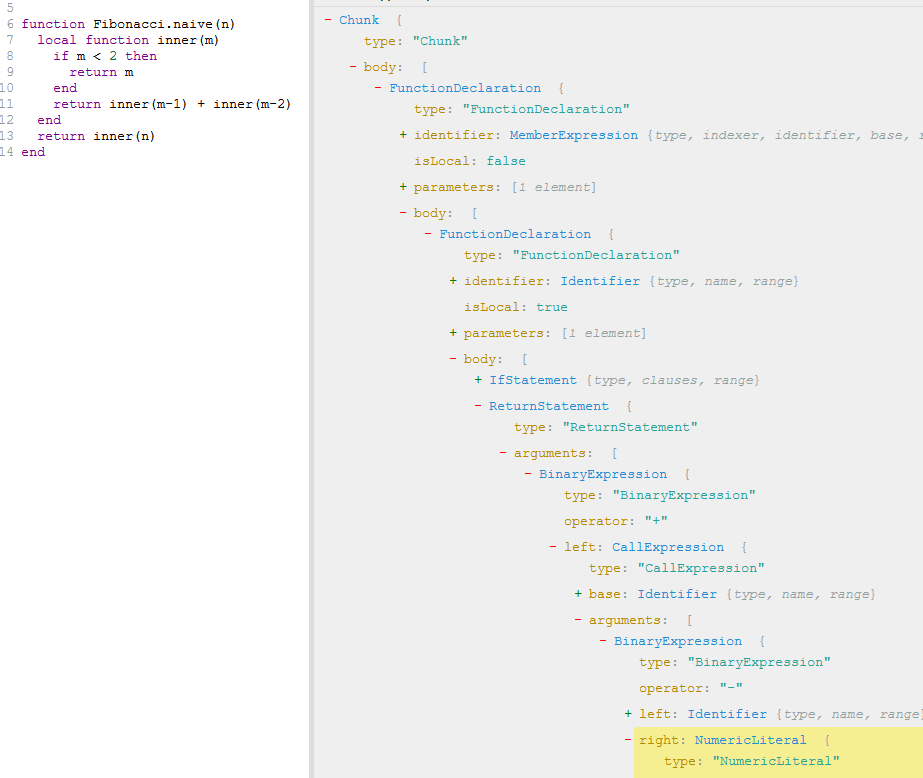
\includegraphics[scale=0.6]{images/ast_lua.png}
\caption{AST isečka koda pisanog u programskom jeziku Lua. Prikazano putem \url{https://astexplorer.net/}}
\label{fig:ASTLua}
\end{figure}

\begin{figure}[h!]
\centering
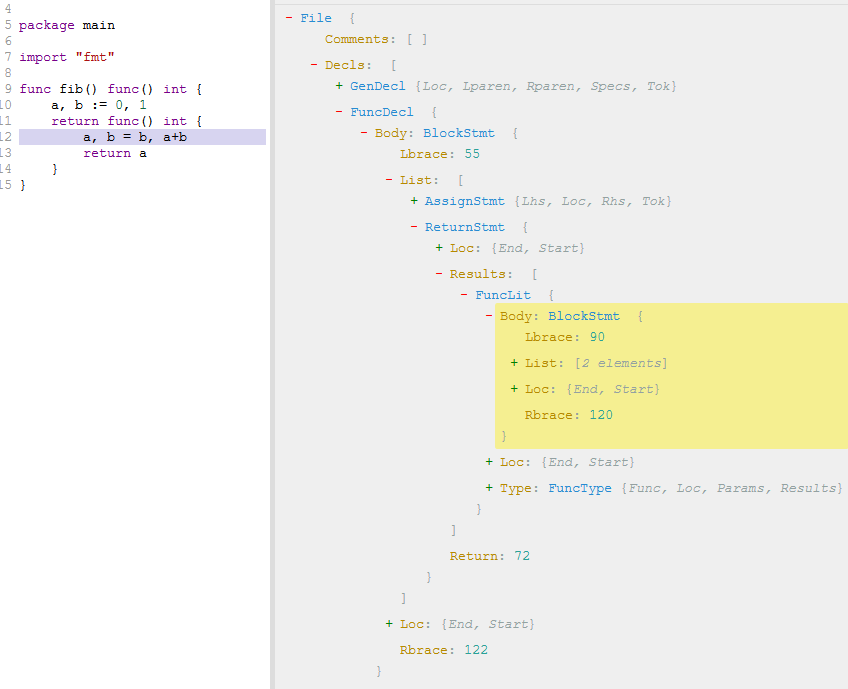
\includegraphics[scale=0.7]{images/ast_go.png}
\caption{AST isečka koda pisanog u programskom jeziku Go. Prikazano putem \url{https://astexplorer.net/}}
\label{fig:ASTGo}
\end{figure}

Kako bi se kreirala smislena apstrakcija stabla parsiranja, potrebno je identifikovati bitne informacije u stablu parsiranja ali i koncepte same gramatike koji su ponovno upotrebljivi. Najjednostavnije rešenje je mimikovati čvorove stabla parsiranja, ukoliko su gramatička pravila kreirana tako da oslikaju koncepte jezika koji gramatika definiše. Na primer, ukoliko u gramatici imamo pravilo \texttt{deklaracija} sa alternativama \texttt{deklaracijaPromenljive} i \texttt{deklaracijaFunkcije}, možemo kreirati apstraktni koncept \texttt{Deklaracija} sa konkretizacijama \texttt{DeklaracijaPromenljive} i \texttt{DeklaracijaFunkcije}. Kako se definišu deklaracije promenljivih i funkcija zavisi dalje od definicija pravila \texttt{deklaracijaPromenljive} i \texttt{deklaracijaFunkcije}. Naravno, nije uvek moguće primeniti ovakav postupak. Takođe, nekada u gramatici definišemo pomoćna pravila kako bismo se izborili sa rekurzijom ili izbegli neke tipove rekurzije --- ta pravila ne bi trebalo da imaju odgovarajuće tipove u opštoj apstrakciji. 

Pošto su u pitanju gramatike programskih jezika, onda je jasno da dosta različitih gramatika dele slične koncepte i da je moguće definisati tipove čvorova koji odgovaraju tim konceptima. Neki od njih mogu biti: naredba, izraz, deklaracija, poziv funkcije, dodela itd. Može se uočiti i hijerarhija između navedenih koncepata, međutim poziv funkcije se može smatrati kao samostalna naredba ali može biti i deo izraza. Dakle, prilikom definisanja hijerarhije ne treba dozvoliti nešto što nema smisla (npr. ako je dozvoljeno višestruko nasleđivanje i poziv funkcije je i naredba ali i izraz, onda se izrazi u kojima figurišu pozivi funkcija sastoje od više naredbi.).

Osim naredbi i izraza (koje vezuju operatori), kao osnovnih koncepata imperativnih jezika, deklaracije se ne pojavljuju u skript jezicima zbog slabe tipiziranosti. Moguće je, međutim, posmatrati i promenljive u kodovima skript jezika kao promenljive deklarisane neposredno pre trenutka njihove upotrebe --- detaljnije opisano u \ref{subsec:MyASTDeclarationNodes}. Što se tiče njihovog tipa, može biti dozvoljena promena istog, ili, kako je izabrano u ovom radu, biće iskorišćen specijalni tip od kog potiču svi ostali tipovi.

\begin{figure}[h!]
\centering
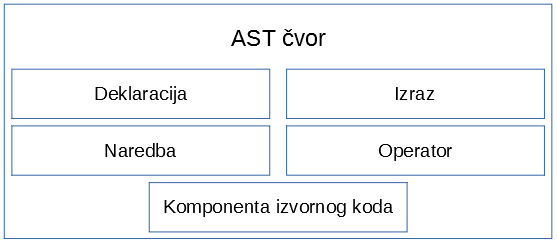
\includegraphics[scale=0.6]{images/nodes.png}
\caption{Prikaz osnovnih vrsta AST čvorova.}
\label{fig:ASTNode}
\end{figure}

Na slici \ref{fig:ASTNode} se mogu videti osnovni tipovi AST čvorova zasnovani na konceptima opisanim iznad. U nastavku će po odeljcima biti detaljnije opisan svaki od prikazanih tipova.

\subsection{Čvorovi deklaracija}
\label{subsec:MyASTDeclarationNodes}

Kao što je opisano u odeljku \ref{sec:Paradigms}, u striktno tipiziranim proceduralnim jezicima promenljive i funkcije koje se koriste se moraju deklarisati pre trenutka njihovog korišćenja. Prateći kvalifikatori (statičnost, konstantnost itd.) i modifikatori pristupa (javni, privatni itd.) će se u nastavku nazivati \emph{specifikatori deklaracije} (engl. \emph{declaration specifiers}). Nakon specifikatora deklaracije dolazi konkretan \emph{deklarator}, koji ima specifičan oblik u zavisnosti od toga šta se deklariše. Oba imena su uzeta po uzoru na imena pravila gramatike programskog jezika C. 

Veliki broj proceduralnih jezika dozvoljava deklarisanje više promenljivih odjednom koje dele iste specifikatore deklaracije. Stoga specifikatore neće pratiti jedan deklarator, nego \emph{lista deklaratora}. Takođe, deklaratori u listi ne moraju biti samo deklaratori promenljivih --- moguće je deklarisati i nizovnu promenljivu zajedno sa deklaracijama običnih promenljivih. Na slici \ref{fig:DeclarationParts} se može videti dekompozicija deklaracije promenljive i niza u različitim proceduralnim programskim jezicima a na slici \ref{fig:DeclarationNodes} uočena hijerarhija sa podvrstama deklaratora.

\begin{figure}[h!]
\centering
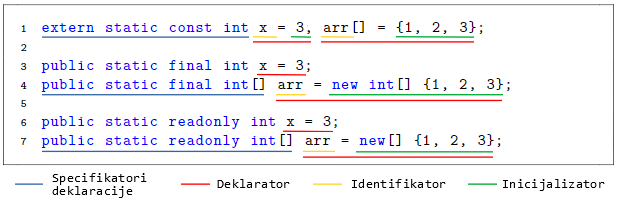
\includegraphics[scale=0.8]{images/declaration_decomposition.png}
\caption{Delovi deklaracije promenljive i niza prikazani na isečcima koda pisanog u programskim jezicima C, Java i C\#.}
\label{fig:DeclarationParts}
\end{figure}

\begin{figure}[h!]
\centering
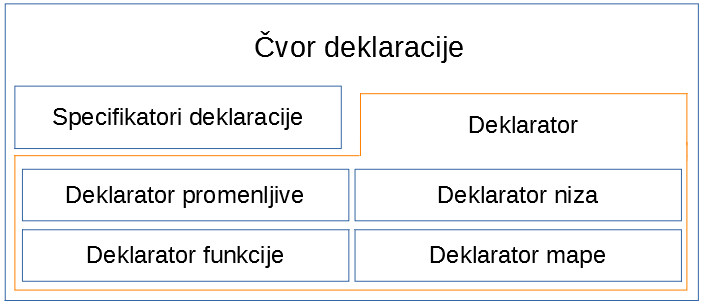
\includegraphics[scale=0.5]{images/declaration_nodes.png}
\caption{Prikaz vrsti AST čvorova deklaracije.}
\label{fig:DeclarationNodes}
\end{figure}

Kao što je prikazano na slici \ref{fig:DeclarationParts}, specifikatori deklaracije pokrivaju kvalifikatore, specifikatore pristupa i ime tipa. Pošto se pravi zajednička apstrakcija, potrebno je uočiti ekvivalenetne ključne reči u različitim programskim jezicima --- u primeru sa slike to su \texttt{const}, \texttt{final} i \texttt{readonly}. Imena tipova u programskim jezicima Java i C\# uzeta su po uzoru na programski jezik C, tako da tu ne vidimo razlike. U opštem slučaju, moguće je definisati mapiranje imena tipa u apstraktni tip. Ukoliko, na primer, posmatramo tipove koji predstavljaju realne brojeve, osim tipova \texttt{float} i \texttt{double}, postoji i tip \texttt{decimal}\footnote{Tip \texttt{decimal} predstavlja 128-bitni realan broj sa povećanom veličinom mantise a smanjenom veličinom eksponenta u odnosu na tip \texttt{double}. Koristi se pri numeričkm izračunavanjima gde preciznost primitivnih tipova realnih brojeva nije dovoljna.} prisutan u programskom jeziku C\#. Sva tri ova tipa mogu da se posmatraju na istom nivou apstrakcije kao tip realnih brojeva. Za korisnički definisane tipove isto ne može da se primeni.

Deklaratori za proceduralne jezike mogu biti deklaratori promenljive, niza ili funkcije i od toga zavisi njihov sastav. Svi deklaratori moraju sadržati informaciju o idenfitikatoru. Ukoliko je reč o deklaratoru niza, dodatno se očekuje i oznaka za niz (obično par srednjih zagrada --- \texttt{[]}) i opcioni izraz koji predstavlja dimenziju niza, obično unutar oznake niza. Ukoliko je reč o deklaratoru funkcije, pored identifikatora se očekuje i lista parametara funkcije obično navedena unutar para običnih zagrada. Lista parametara funkcije se može posmatrati rekurzivno --- svaki parametar se može posmatrati kao varijanta deklaracije --- sadrži specifikatore deklaracije (koji uključuju i tip) i deklarator, s tim što u ovom slučaju nije dozvoljeno da taj deklarator bude deklarator funkcije (pošto funkcije nisu građani prvog reda u imperativnoj paradigmi). 

Deklaratori promenljive i niza mogu dodatno sadržati i \emph{inicijalizator}. Inicijalizator možemo posmatrati kao opcioni izraz u slučaju deklaratora promenljive. U slučaju deklaratora niza, inicijalizator može biti lista izraza. Deklaratori funkcije ne mogu imati inicijalizatore.

U skript jezicima su uobičajeno podržane strukture podataka kao što su skupovi i mape. Stoga, kako bi se i mape mogle predstaviti apstraktno, dodat je tip deklaratora koji predstavlja deklarator mape. Mapa se sastoji od skupa ključeva pri čemu je svakom ključu dodeljena vrednost ne nužno istog tipa kao što je tip ključa. Mape postoje i u proceduralnim jezicima, ali ključna razlika je ta što tipovi u skript jezicima nisu striktni --- ključevi međusobno, ali i vrednosti mogu biti različitog tipa. Vredi naglasiti da se mape mogu porediti sa objektima određenih klasa --- svaki objekat se može serijalizovati u mapu gde su ključevi imena javnih atributa klase a vrednosti su vrednosti javnih atributa objekta koji se serijalizuje. Neki jezici (kao što je Python), imaju funkcije koje od objekta vraćaju baš ovakvu mapu. Ova ideja se dalje može proširiti kako bi se serijalizovale i metode klase, označila statička i privatna polja kao i sačuvale informacije o definisanim konstruktorima. Zatim je moguće porediti mape definisane u skript jezicima sa objektima iz proceduralnih jezika.

Na slici \ref{fig:MyASTExampleCDeclaration} se mogu videti kreirani AST za nekoliko deklaracija pisanih u programskom jeziku C a na slici \ref{fig:MyASTExampleLuaDeclaration} se može isto videti demonstracija \emph{automatske deklaracije} promenljivih za skript programski jezik Lua. Naime, pre prvog pojavljivanja identifikatora veštački će biti deklarisan taj identifikator, kako bi razlika između apstrakcija dobijenih iz proceduralnih i skript jezika bila što manja. U ovom slučaju će se deklaracija i dodela spojiti u deklaraciju sa inicijalizatorom.

\begin{figure}[h!]
\begin{lstlisting}
extern int y = 3;
static int arr[5] = { 1 };
\end{lstlisting}
\centering
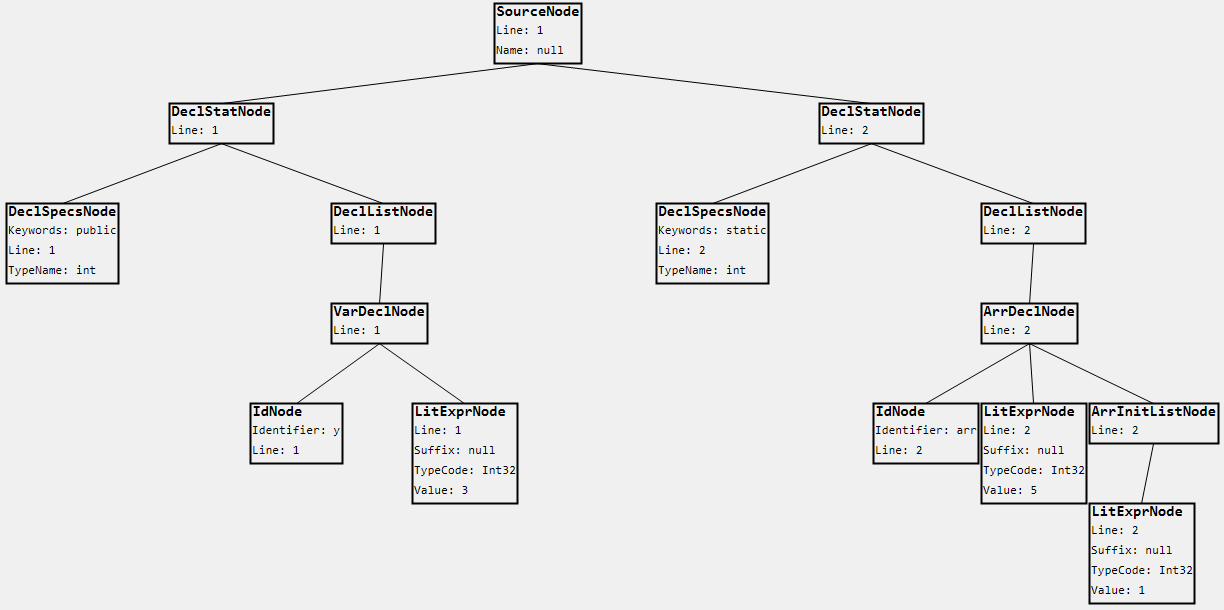
\includegraphics[scale=0.48]{images/c_ast_decl2.png}
\caption{Primer deklaracije promenljive i niza u programskom jeziku C i odgovarajući AST.}
\label{fig:MyASTExampleCDeclaration}
\end{figure}

\begin{figure}[h!]
\begin{lstlisting}
arr = { 1, 2 }
dict = { a = 1 }
\end{lstlisting}
\centering
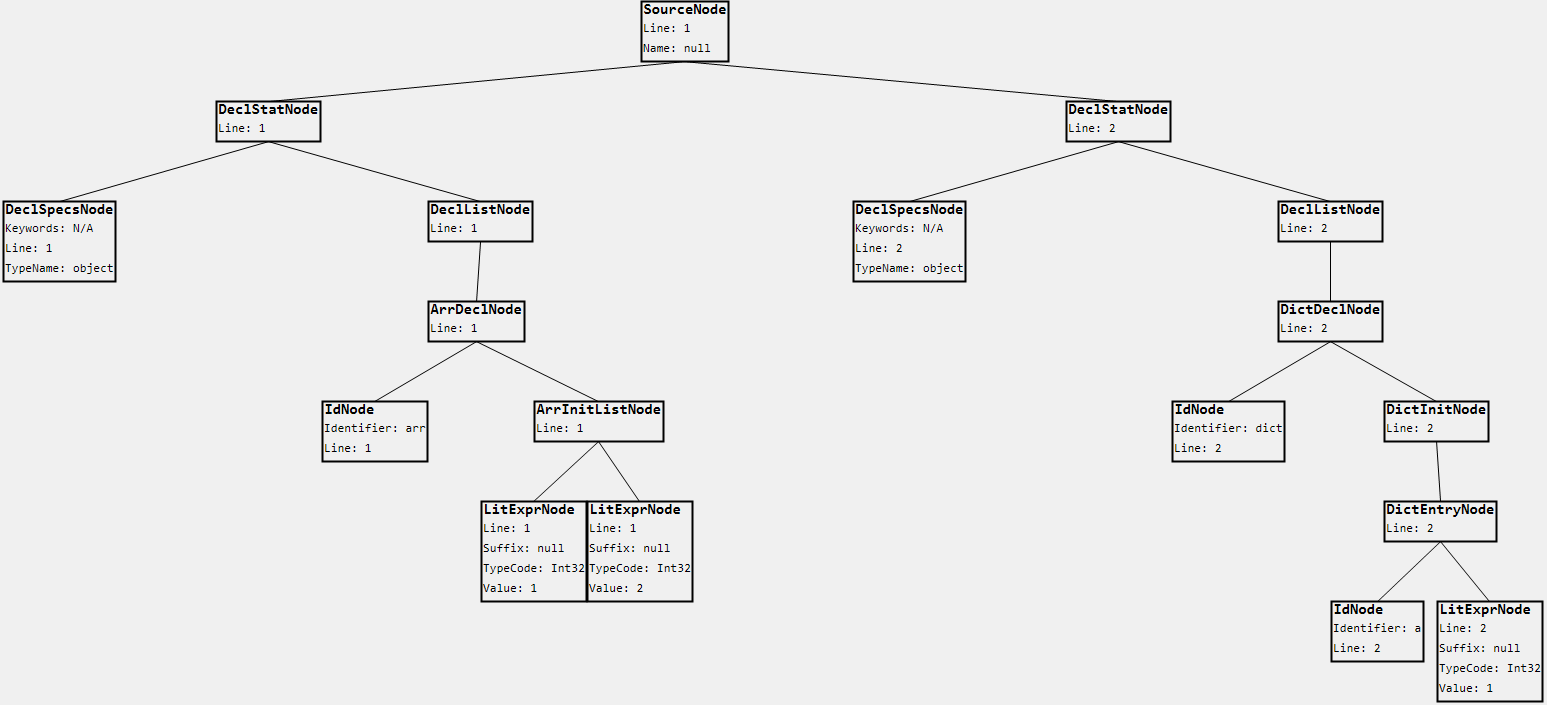
\includegraphics[scale=0.4]{images/lua_ast_decl.png}
\caption{Primer deklaracije promenljive i niza u programskom jeziku Lua i odgovarajući AST.}
\label{fig:MyASTExampleLuaDeclaration}
\end{figure}


\subsection{Čvorovi operatora}
\label{subsec:MyASTOperatorNodes}

Svrha operatora je da vezuju izraze i da tako grade nove izraze. Operator se karakteriše simbolom i \emph{arnošću}, tj. brojem argumenata koje taj operator prima. Na osnovu arnosti, svaki operator se može apstraktno posmatrati kao članica grupe operatora sa istom arnošću. Na slici \ref{fig:OperatorNodes} se može videti hijerarhija operatora korišćena dalje u apstrakciji. Binarni operatori zahtevaju dva operanda i pišu se infiksno, dok unarni zahtevaju jedan operand i pišu se prefiksno. Ternarni operatori koji postoje u nekim programskim jezicima nisu razmatrani jer se mogu posmatrati kao druge strukture\footnote{Na primer, ternarni operator \texttt{?:} prisutan u jezicima zasnovanim na sintaksi programskog jezika C se može zameniti naredbom uslovnog grananja.}. 

\begin{figure}[h!]
\centering
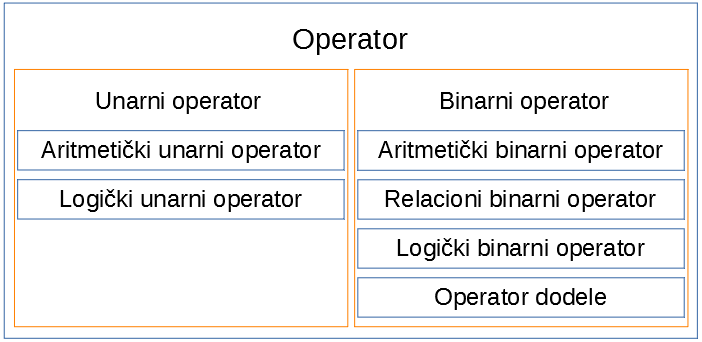
\includegraphics[scale=0.5]{images/operator_nodes.png}
\caption{Podela operatora na osnovu njihove arnosti.}
\label{fig:OperatorNodes}
\end{figure}

Unarni aritmetički operatori su unarni operatori koji figurišu u aritmetičkim izrazima, npr. operator promene znaka, operator bitovske negacije\footnote{Bitovski izrazi se mogu posmatrati kao vrsta aritmetičkih izraza.}, operatori kastovanja ili inkrementiranja odnosno dekrementiranja. Unarni logički operatori su unarni operatori koji figurišu u logičkim izrazima, npr. operator negacije. Možemo sve ove unarne operatore posmatrati apstraktno ukoliko definišemo unarni operator kao strukturu koja definiše unarnu funckiju koja transformiše svoj argument na osnovu logike konkretnog unarnog operatora. Tip argumenta i povratne vrednosti pomenute funkcije zavisi od tipa unarnog operatora --- aritmetički unarni operatori mogu primiti vrednost bilo kog tipa\footnote{Ne postoji ograničenje na brojevne tipove jer se u nekim jezicima operatori mogu predefinisati tako da rade i za korisnički definisane tipove (engl. \emph{operator overloading}).} i vraćaju vrednost proizvoljnog, ne nužno istog tipa; dok unarni logički operatori primaju i vraćaju bulovsku vrednost\footnote{U nekim programskim jezicima postoji implicitna konverzija brojevnih tipova u bulovski tip, što se jednostavno može posmatrati kao poređenje vrednosti po jednakosti sa nulom.}. Koristeći ovaj pristup, nije potrebno praviti novi AST čvor za svaki mogući operator, već je dovoljno da postoji samo jedan čvor koji predstavlja unarni operator. Ovakav pristup odgovara varijanti AST sa regularnošću (videti sliku \ref{fig:ASTVariants}), omogućava opisivanje proizvoljnih operatora i nije vezan za konkretnu programsku paradigmu.

Binarni aritmetički operatori su binarni operatori koji figurišu u aritmetičkim izrazima, npr. operatori koji odgovaraju matematičkim operacijama ali i bitovski binarni operatori. Binarni relacioni operatori su binarni operatori koji figurišu u relacionim izrazima, npr. operatori poretka ($<$, $>$, $\leq$, $\geq$) i poređenja po jednakosti ili različitosti ($=$, $\neq$). Binarni logički operatori su binarni operatori koji figurišu u logičkim izrazima, npr. bulovske operacije ($\wedge$, $\vee$). Slično kao i za unarne operatore, moguće je apstraktno posmatrati sve binarne operatore tako što ih definišemo kao strukturu koja definiše binarnu funkciju koja transformiše argumente na osnovu logike konkretnog binarnog operatora. Tip argumenata i povratne vrednosti te funkcije zavisi od tipa binarnog operatora, kao i u slučaju unarnih operatora --- aritmetički binarni operatori primaju dva argumenta proizvoljnog tipa i vraćaju rezultat proizvoljnog, ne nužno istog tipa; relacioni binarni operatori primaju iste tipove argumenata kao i aritmetički binarni operatori, međutim povratna vrednost mora biti bulovskog tipa; dok logički binarni operatori zahtevaju da argumenti i povratna vrednost budu bulovskog tipa. Pritom, na prvi pogled nije jasno kako se operator dodele može uklopiti u ovaj šablon ali, na osnovu toga da je dodela zapravo sporedni efekat i da se posmatra kao izraz čija je vrednost jednaka vrednosti izraza sa desne strane operatora, može se primeniti isti princip kao i za aritmetičke binarne izraze. Neki programski jezici dozvoljavaju i složene operatore dodele, koji se mogu dekomponovati na više jednostavnijih izraza.

\subsection{Čvorovi izraza}
\label{subsec:MyASTExpressionNodes}

Izraz, kao što se može videti na primeru gramatike sa slike \ref{fig:ANTLRExpressions}, se definiše rekurzivno i izraze mogu proširiti razni operatori. Na slici \ref{fig:ExpressionNodes} se mogu videti tipovi apstraktnih konstrukcija koje će se koristiti da bi se predstavili izrazi. Dodatno, za vezivanje izraza će se koristiti apstrakcije operatora definisane u prethodnom odeljku.

\begin{figure}[h!]
\centering
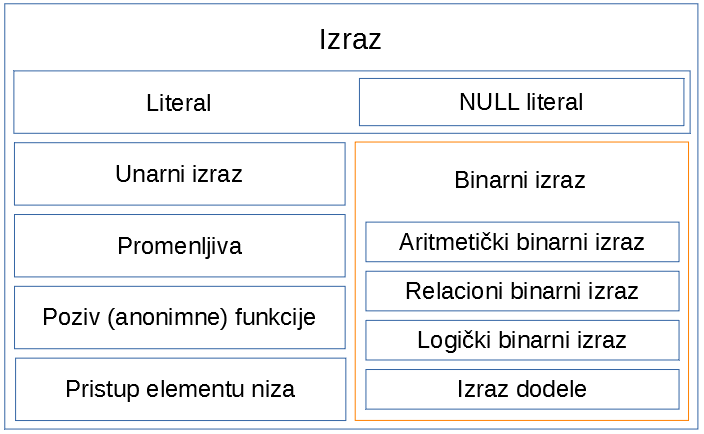
\includegraphics[scale=0.5]{images/expression_nodes.png}
\caption{Vrste čvorova izraza.}
\label{fig:ExpressionNodes}
\end{figure}

Najjednostavniji izraz predstavljaju konstante ili \emph{literali}. Literali mogu biti brojevne konstante, karakterske konstante ili konstantne niske. Literali često mogu imati i sufiks (najčešće za brojevne literale), koji određuje tip literala u slučajevima gde postoji dvosmislenost. Na primer, literal $5$ možemo posmatrati kao 32-bitni ceo broj ili kao 64-bitni ceo broj (ali i kao realan broj, ako ne zahtevamo da realne brojeve moramo pisati u nepokretnom ili pokretnom zarezu). Da bi se ova dvosmislenost uklonila, možemo eksplicitno naznačiti da se govori o 64-bitnom celom broju dodavanjem sufiksa \texttt{L}, ako je u pitanju programski jezik C ili njemu slični jezici. Takođe, pošto nezanemarljiv broj programskih jezika dozvoljava rad sa pokazivačima ili neposredno koristi alokaciju memorije za kreiranje objekata, uobičajeno je korišćenje prazne adrese kao specijalne vrednosti (\texttt{null} ili \texttt{nil}). Za ovu specijalnu vrednost je moguće kreirati poseban tip literala, jer ovaj literal može biti bilo kog tipa koji nije primitivni tip.

Osim literala, samostalne promenljive mogu predstavljati validan izraz, u kom slučaju je vrednost izraza trenutna vrednost te promenljive. Slično važi i za indeksni pristup nizu\footnote{Isto važi i za bilo koju drugu kolekciju, ukoliko je nad njom definisan operator indeksnog pristupa. Predefinisanje ovog operatora nije razmatrano u ovom radu.}. U slučaju indeksnog pristupa, potrebno je navesti izraz čija vrednost označava indeks (to ne mora biti jednostavni literal). Postoje smislena ograničenja šta sve sme da se nađe unutar izraza koji predstavlja indeks elementa niza tako da to semantički ima smisla, ali se na ovom nivou ne bavimo semantičkom analizom. 

Unutar izraza se mogu naći i pozivi funkcija. Naravno, pretpostavljamo da funkcija ima povratnu vrednost, koja će se iskoristiti nakon poziva funkcije u kontekstu iz kojeg je ona pozvana. Pod uticajem funkcionalne paradigme, veliki broj programskih jezika dozvoljava definisanje anonimnih (lambda) funkcija, čija se definicija može smatrati izrazom koji se može dodeliti nekom simbolu. Stoga se i anonimne funkcije mogu smatrati validnim izrazima. 

Operatori opisani u \ref{subsec:MyASTOperatorNodes} mogu vezati sve tipove iznad i formirati složenije izraze. U zavisnosti od broja izraza koje operator vezuje, izraze možemo podeliti na unarne i binarne. Unarne izraze nadograđuju unarni operatori dok su binarni izrazi dobijeni primenom binarnog operatora na dva izraza. U zavisnosti od tipa binarnog operatora (videti sliku \ref{fig:OperatorNodes}), binarne izraze delimo na sličan način. Naravno, svaki od tipova binarnog izraza zahteva odgovarajući tip binarnog operatora. Slično se može uraditi i za unarne izraze, ali takođe i napraviti podela na prefiksne i postfiksne unarne izraze. S obzirom da je cilj napraviti opšti AST, činjenica da li je unarni operator prefiksni ili postfiksni nije od suštinskog značaja, pogotovo ukoliko se uzme u obzir da dva programska jezika mogu imati unarne operatore sa istom semantikom ali različitom pozicijom u odnosu na operand --- u jednom jeziku taj operator može biti prefiksni a u drugom postfiksni. Kako bi poređenje ovakvih operatora funkcionisalo bez obzira na njihovu poziciju u odnosu na operand, u ovom radu nije pravljena podela na prefiksne i postfiksne unarne operatore.

Na slici \ref{fig:MyASTExampleExpressions} se mogu videti kreirani AST za izraz \texttt{(3 + 5) << f(4)}. Ovaj izraz poprima isti oblik bez obzira na to koji je programski jezik u pitanju, ali iako se sintaksa bude razlikovala ili operatori budu imali drugi simbol, logika operatora opisana putem funkcije će ostati ista.

\begin{figure}[h!]
\centering
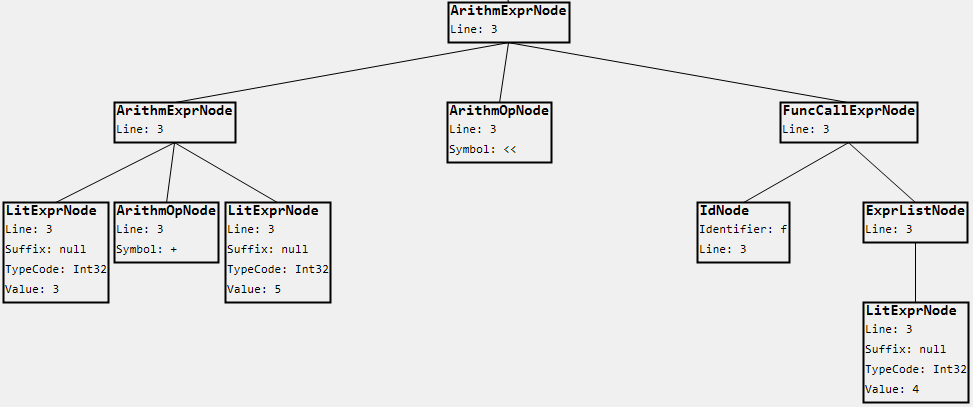
\includegraphics[scale=0.6]{images/ast_expr.png}
\caption{AST generisan od izraza \texttt{(3 + 5) << f(4)}.}
\label{fig:MyASTExampleExpressions}
\end{figure}

\subsection{Čvorovi naredbi}
\label{subsec:MyASTStatementNodes}

Naredbe su najkomplikovanije za apstrahovanje zbog njihove raznovrsnosti. Programski jezici često uvode nove sintaksičke strukture i naredbe koje nisu do tada viđene u ostalim jezicima. Uprkos svemu tome, ipak je moguće uočiti neke sličnosti sa već postojećim konceptima i svesti ih na isti nivo. Na slici \ref{fig:StatementNodes} se mogu videti tipovi apstraktnih konstrukcija koje će se koristiti da bi se predstavile naredbe.

\begin{figure}[h!]
\centering
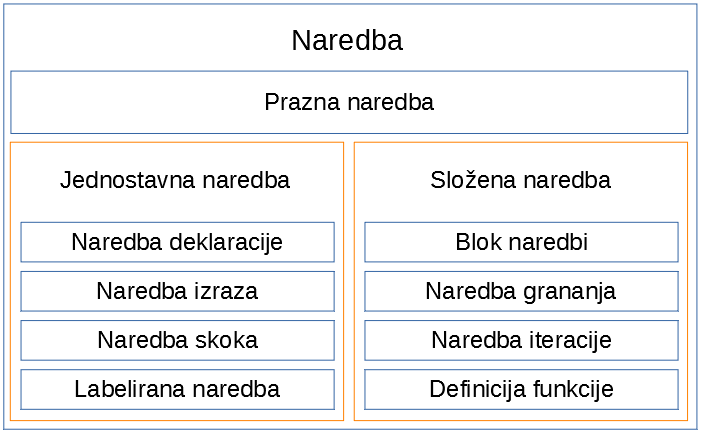
\includegraphics[scale=0.5]{images/statement_nodes.png}
\caption{Vrste čvorova naredbi.}
\label{fig:StatementNodes}
\end{figure}

Veliki broj programskih jezika podržava praznu naredbu, sa semantikom ne izvršavanja nikakvih operacija. U programskim jezicima koji su zasnovani na sintaksi jezika C, praznu naredbu navodimo samo korišćenjem simbola za kraj naredbe (\texttt{;}), dok u programskom jeziku Python koristimo ključnu reč \texttt{pass}. 

Naredbe su podeljene na \emph{jednostavne} i \emph{složene}, koje se sastoje od više drugih naredbi. Primer jednostavne naredbe može biti deklaracija promenljive, dok primer složene naredbe može biti definicija funkcije koja se sastoji od više jednostavnih deklaracija ali možda i drugih složenih naredbi kao što su grananja i petlje.

Jednostavne naredbe uključuju naredbe deklaracije i izraza. Razlog zašto se deklaracije i izrazi opet pojavljuju je taj što izrazi sami po sebi mogu biti deo drugih naredbi. Ukoliko se naredba sastoji samo od izraza, onda nju zovemo naredbom izraza. Primer može biti izraz dodele --- vrednost izraza dodele se može koristiti u drugim izrazima ali, ukoliko samo želimo da izvršimo dodelu i ništa više u okviru iste naredbe, onda izraz dodele "umotavamo" u naredbu izraza. Slično važi i za deklaracije, ukoliko razmotrimo idiomsku \texttt{for} petlju (od standarda C99) --- moguće je deklarisati promenljive koje se koriste unutar ciklusa ali to nije naredba deklaracije već deklaracija koja se koristi unutar druge naredbe. 

Naredbe se mogu označiti, po uzoru na koncept \emph{labele} u imperativnim jezicima --- identifikatorom koji označava lokaciju u izvornom kodu. Labele se u imperativnim jezicima najviše koriste da bi se izvršili skokovi na određene lokacije u kodu ali su takođe prisutne i u proceduralnim jezicima (npr. kroz naredbu višestrukog grananja --- \texttt{switch} ili u nekim jezicima \texttt{case}). Labelirana naredba se sastoji od naredbe i identifikatora koji predstavlja labelu. 

Naredbe skoka se koriste obično u paru sa labeliranim naredbama, ali to ne mora uvek biti slučaj. Iako ove čvorove koristimo da bismo predstavili naredbe skoka prisutne u imperativnim jezicima, one predstavljaju i naredbe prekida (\texttt{break} ili \texttt{continue}) ili povratka vrednosti funkcije (\texttt{return}). U slučaju da je u pitanju skok na određenu labelu, onda se sastoji i od identifikatora koji predstavlja labelu na koju se skače. Ukoliko je u pitanju naredba prekida, nisu potrebne nikakve dodatne informacije (mada se i u tom slučaju može iskoristiti činjenica da su u pitanju skokovi pa se može labelirati petlja na koju se odnosi naredba prekida). U slučaju povratka vrednosti funcije, sadrži opcioni izraz čija vrednost predstavlja povratnu vrednost funkcije.

Složene naredbe se sastoje od više drugih naredbi (ne nužno samo od jednostavnih). Često je potrebno izvršiti više naredbi u okviru jednog konteksta i za to se koristi blok naredba. Blok naredba grupiše više drugih naredbi u jednu. Blok naredba se u proceduralnim jezicima, obično navodi eksplicitno --- recimo za programski jezik C pomoću velikih zagrada (\texttt{\{\}}). Za skript jezike često nije potrebna nikakva eksplicitna oznaka već se blok naredba prepoznaje implicitno ili se navodi korišćenjem različitih nivoa indentacije (Python). Neki skript jezici, na primer Lua, zahtevaju eksplicitno navođenje ključnih reči pre početka i nakon kraja blok naredbe ukoliko je ona deo složenije naredbe.

Naredbe uslovnog grananja se sastoje od \emph{uslova}, koji može biti relacioni ili logički izraz, naredbe koja se vrši ukoliko je uslov ispunjen (\emph{then} grana), i opciono naredbe koja se izvršava ako uslov nije ispunjen (\emph{else} grana). Rezultat uslovnog izraza, iako mora biti istinitosna vrednost, je dozvoljeno da bude bilo kog tipa (dakle nema ograničenja samo na relacione i logičke izraze) iz razloga što određeni programski jezici dozvoljavaju automatsku konverziju brojevnih tipova u logički (C). Štaviše, nekada je moguća i implicitna konverzija određenih tipova u logički tip definisanjem implicitnih operatora konverzije (C\#). Zato će u apstrakciji uslov biti bilo koji izraz. Što se \emph{then} i \emph{else} grana tiče, one mogu biti bilo koje naredbe, ali zarad konzistentnosti će obe biti blokovi naredbi. Na slici \ref{fig:MyASTExampleStatement} se može videti AST za naredbu grananja.

\begin{figure}[h!]
\begin{lstlisting}
do                               something()
    something()                  while (condition) do
while (condition)                    something()
\end{lstlisting}
\begin{lstlisting}
repeat                           something()
    something()                  while (not condition) do
until (condition)                    something()
\end{lstlisting}
\caption{Procedura svođenja ređih tipova petlji (levo) na \emph{while} petlju (desno) prikazana u pseudo-jeziku.}
\label{fig:ASTIterationStatements}
\end{figure}

Naredbe iteracije imaju raznovrsni oblik u programskim jezicima. Najčešće podržane naredbe iteracije su \emph{for} i \texttt{while} petlje. U opštem slučaju, dovoljno je koristiti samo jedan tip petlji, ali zarad jednostavnosti i prisutnosti ovih tipova u velikoj većini programskih jezika oba će biti podržana. Ostali tipovi petlji, kao što su \emph{do-while} ili \emph{repeat-until} petlje, će se svoditi na njih. \emph{do-while} petlja se može svesti na \emph{while} petlju jednostavnim ponavljanjem tela petlje pre same petlje i kreiranjem obične \emph{while} petlje sa istim uslovom i telom. Slično se može uraditi i za \emph{repeat-until} petlju, s tim što je potrebno samo negirati uslov u dobijenoj \emph{while} petlji. Ovaj proces je ilustrovan na slici \ref{fig:ASTIterationStatements}. 

\begin{figure}[h!]
\centering
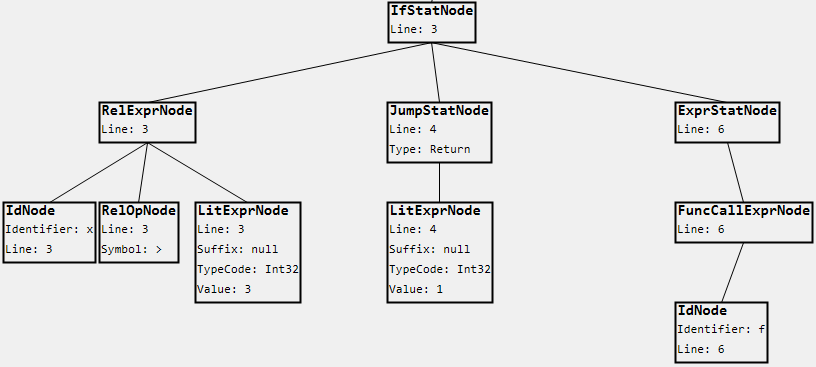
\includegraphics[scale=0.7]{images/ast_stat.png}
\caption{AST naredbe grananja.}
\label{fig:MyASTExampleStatement}
\end{figure}


